% -*- coding: utf-8 -*-
% !TEX encoding = UTF-8 Unicode
% !TEX root =  main.tex

\chapter{Auswertung der Simulationsergebnisse}
\label{chap:ergebnisse-foc}

In diesem Kapitel sollen die Ergebnisse der durchgeführten Simulation aus den Kapitel~\ref{cha:regelungpmsm} diskutiert werden.
%Dabei werden dem Leser Simulationsergebnisse und Probleme gezeigt, diese konnten aufgrund des Zeitaufwandes nicht mehr gelöst werden.
Zu den ausgewählten Lösungsverfahren (s.~h.~Abschnitt~\ref{sec:parameter}) wurde das Runge-Kutta Verfahren mit fester Schrittweite gewählt.

\section{Model and simulation parameter}\label{sec:parameter}

Wie schon in der Einleitung dargestellt, wurde das Runge-Kutta\footnote{Nach Carl Runge und Martin Wilhelm Kutta benannt.} Verfahren gewählt.
Dieses Verfahren ist ein sog. Einzelschrittverfahren zur näherungsweisen Lösung von Anfangswertproblemen in der numerischen Mathematik.
Gegeben sei das Anfangswertproblem

\begin{align}
	y'(t) = f(t,y(t)), y(t_\x{0})=y_\x{0}, y: \mathbb{R}\rightarrow\mathbb{R}^{d}
\end{align}

mit exakter Lösung $y(t)$.
Die exakte Lösung kann im Allgemeinen nicht angegeben werden, weshalb man sich mit einer Näherung, wie Runge-Kutta-Verfahren annährt.
Die $s$-stufigen Runge-Kutta-Verfahren sind Einschrittverfahren, die durch Ausdrücke der folgenden Art gegeben sind

\begin{align}
	y_{n+1} = y_n + h \sum_{j=1}^{s}{b_j k_j}
\end{align}

Dabei bezeichnet $h$ die Schrittweite zwischen den aufeinanderfolgenden Stützstellen $t_n$ und $t_{n+1}$.
Die Koeffizienten $b_j$ definieren das jeweilige Verfahren und können als Quadraturformel für das Integral

\begin{align}
	\int_{t_n}^{t_{n+1}}{f(t,y(t))dt}
\end{align}

interpretiert werden.
Die Größen $k_j$ bezeichnet man als Zwischenschritt, sie entsprechen Auswertungen der rechten Seite von $f$ an bestimmten Stellen.
Die Steuerung der Schrittweite $h$ ist von besonderem Interesse.
Man kann sich leicht vorstellen, dass die Funktion in Bereichen, in denen nur geringe Änderungen zwischen $y_{n+1}$ und $y_n$ vorliegen, mit weniger Rechenschritten auskommt, als in solchen, in den schnelle Änderungen vorliegen.\footnote{Vgl.~W.\ Kutta: \enquote{Beitrag zur näherungsweisen Integration totaler Differenzialgleichungen}, Z. Math. Phys., Bd. 46, 1901, S.~425--453}\footnote{Vgl.~C.\ Runge: \enquote{Über die numerische Auflösung von Differenzialgleichungen}, Math. Annalen, Bd. 46, 1895, S.~167--178, Online \url{http://gdz.sub.uni-goettingen.de/dms/load/img/?PPN=PPN235181684_0046&DMDID=DMDLOG_0022}}


\begin{table}[h!]
	\centering
	\caption{Model configuration parameters.}
	\label{tab:model-parameter}
	\begin{tabularx}{0.8\textwidth}{ll}
		\toprule
		Beschreibung: & Eingestellter Wert: \\
		\midrule
		Solver options	& Fixed Step\\
		Fixed-step size (fundamental sample time)	& 1e-6 \\
		Solver	& ode4 (Runge-Kutta) \\
		Start time & 0.0 \\
		Stop time & 10.0\\
		Periodic sample time constraint & Unconstrained \\
		Tasking mode for periodic sample times & Auto \\
		\bottomrule
	\end{tabularx}
\end{table}
\begin{table}[h!]
	\centering
	\caption{PMSM model configuration parameter.}
	\label{tab:pmsm-parameter}
	\begin{tabularx}{0.8\textwidth}{ll}
		\toprule
		Beschreibung: & Eingestellter Wert: \\
		\midrule
		Trägheitsmoment $J$ & \SI{0.0890}{\kilogram\square\meter} \\
		Frequenz $f$ & \SI{50}{\hertz}\\
		Induktivität in $d,q$-Richtung ($L_\x{d}=L_\x{q}$) & \SI{0.0085}{\ohm\second}\\
		Polpaarzahl $p$ & 4 \\
		FLussverkettung $\Psi_\x{pm}$ & \SI{0.175}{\volt\second}\\
		Ständerwiderstand $R_\x{1}$ & \SI{0.2}{\ohm}\\
		Drehzahl Vorgabe $n_\x{soll}$ & \SI{500}{\per\minute}\\
		Drehmoment Vorgabe $M_\x{Last}$ & \SI{60}{\newton\meter}\\
		\bottomrule
	\end{tabularx}
\end{table}
\verylongpage
\newpage
\section{Simulationsergebnisse ohne Netz}\label{sec:sim-ohne-netz}

In diesem Abschnitte werden die Ergebnisse der Simulation ohne Netz dargestellt.

\begin{minipage}[t]{0.5\textwidth}
		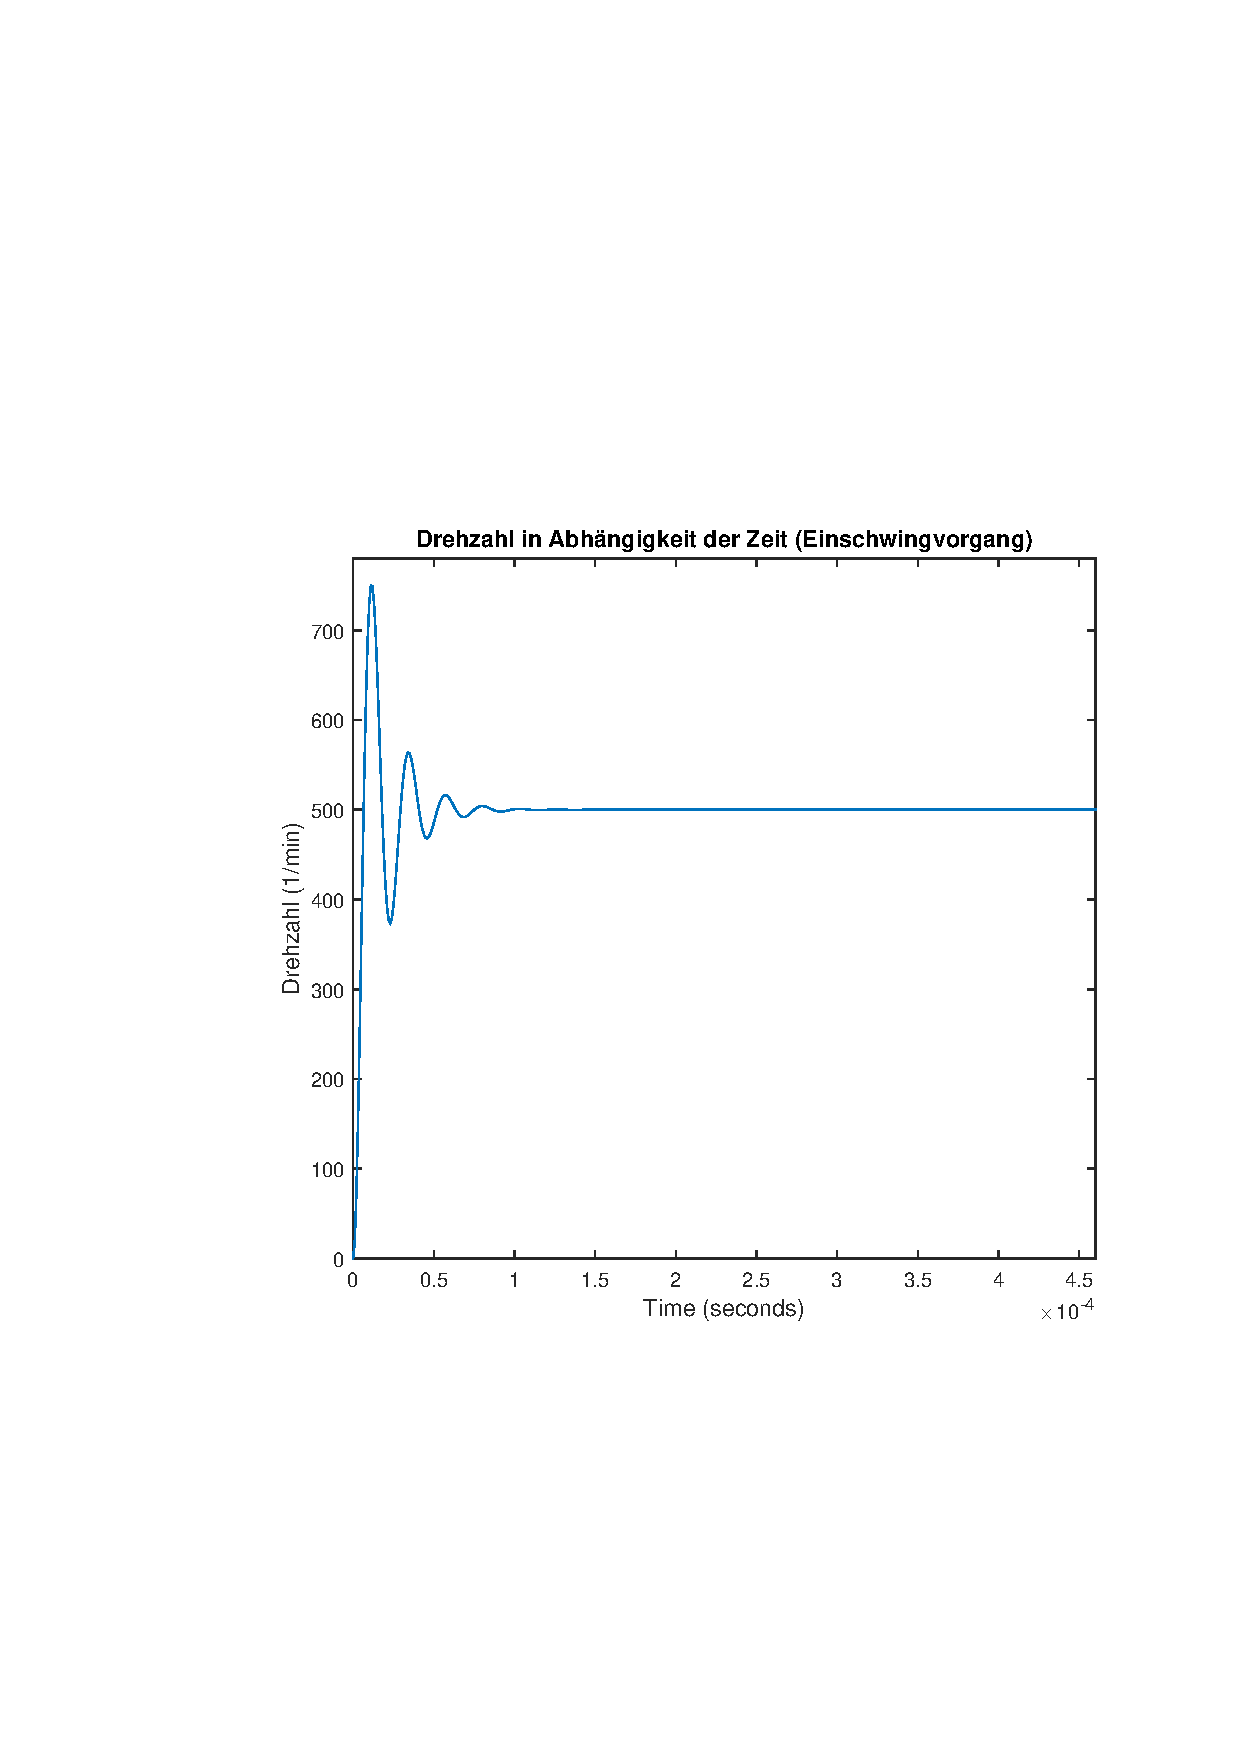
\includegraphics[width=\textwidth]{erg/drehzahl-einschwingvorgang.pdf}
\end{minipage}
\begin{minipage}[t]{0.5\textwidth}
		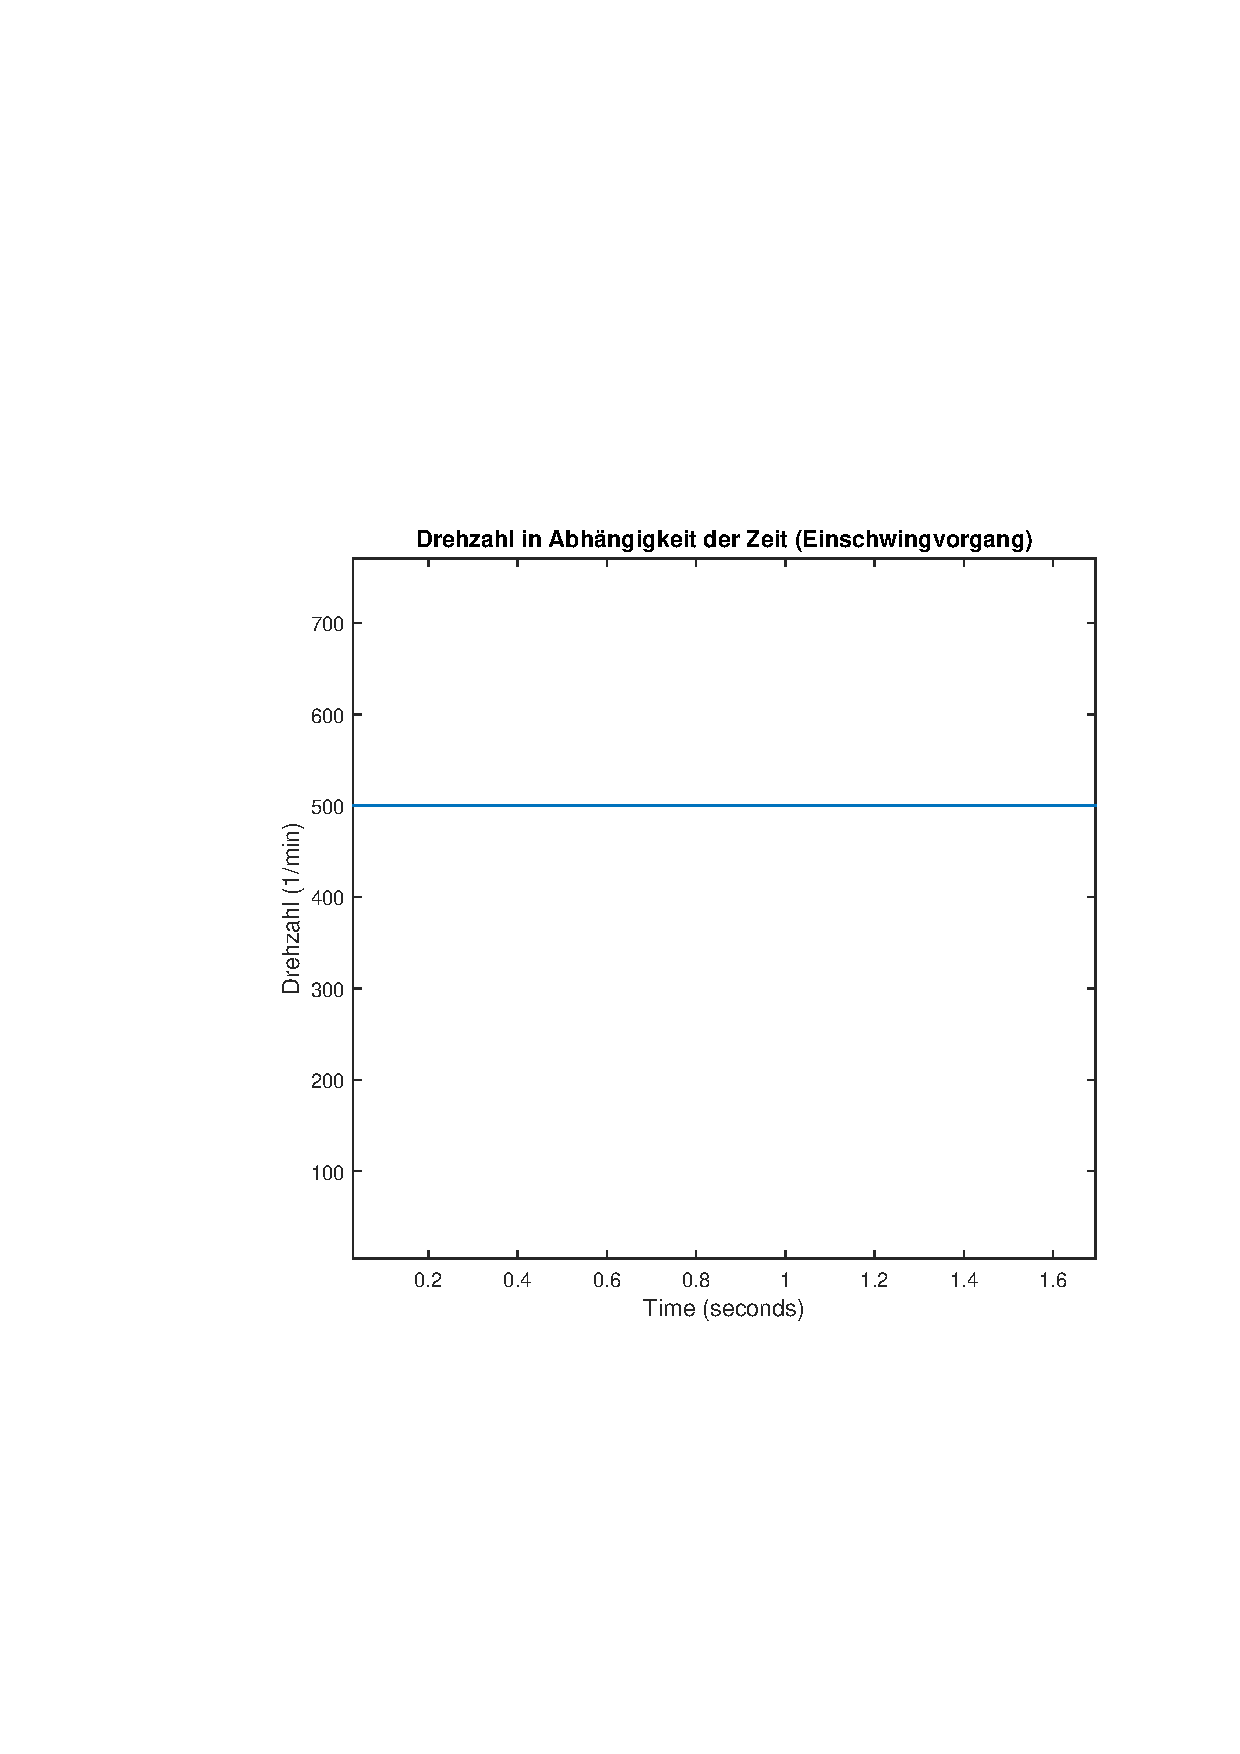
\includegraphics[width=\textwidth]{erg/drehzahl-einschwingvorgang-2.pdf}
\end{minipage}

Wie erwartet schwingt sich die Maschine bei einer Solldrehzahl von \SI{500}{\per\minute} ein.
Nach \SI{3}{\sec} wird ein Lastsprung auf das System draufgegeben, um zu überprüfen, ob die Regelung funktioniert.

\begin{minipage}[t]{0.5\textwidth}
	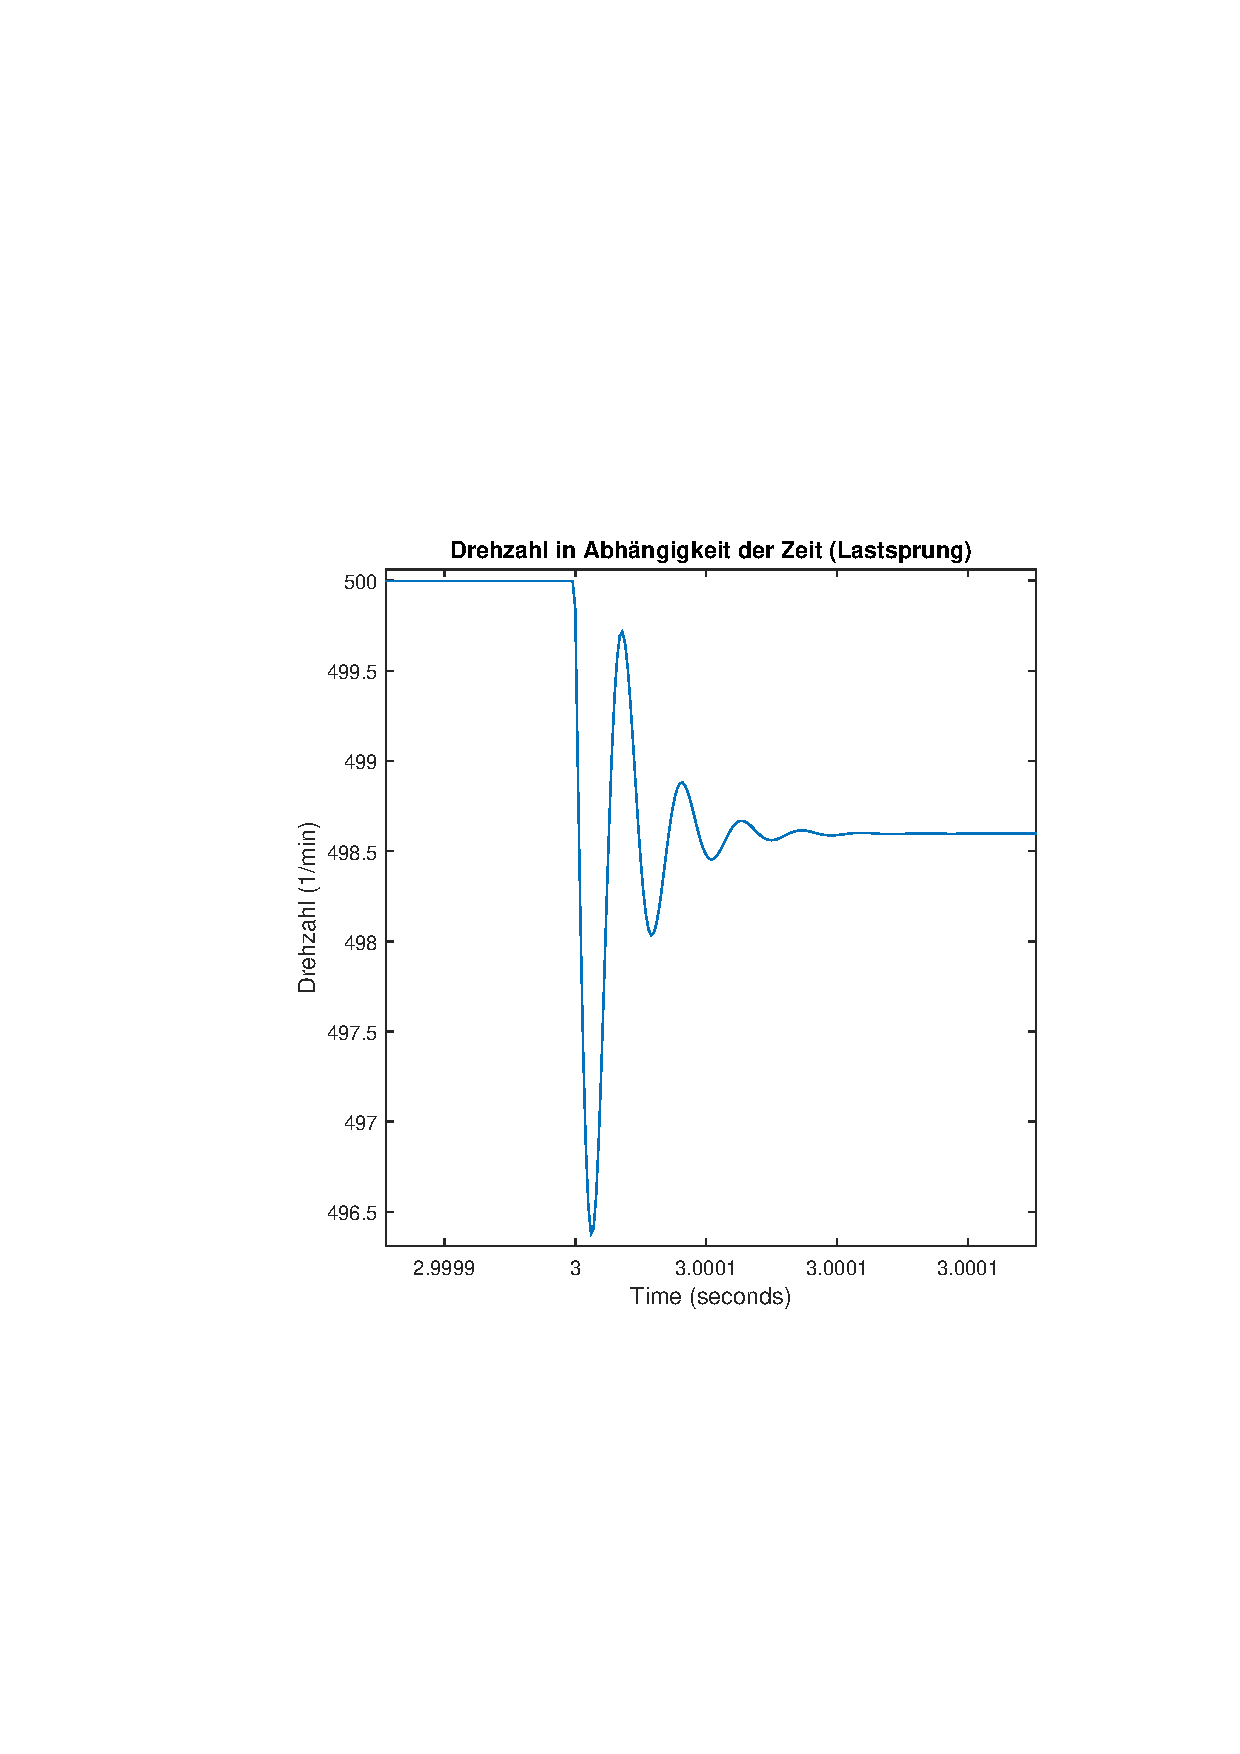
\includegraphics[width=\textwidth]{erg/drehzahl-lastsprung-1.pdf}
\end{minipage}
\begin{minipage}[t]{0.5\textwidth}
	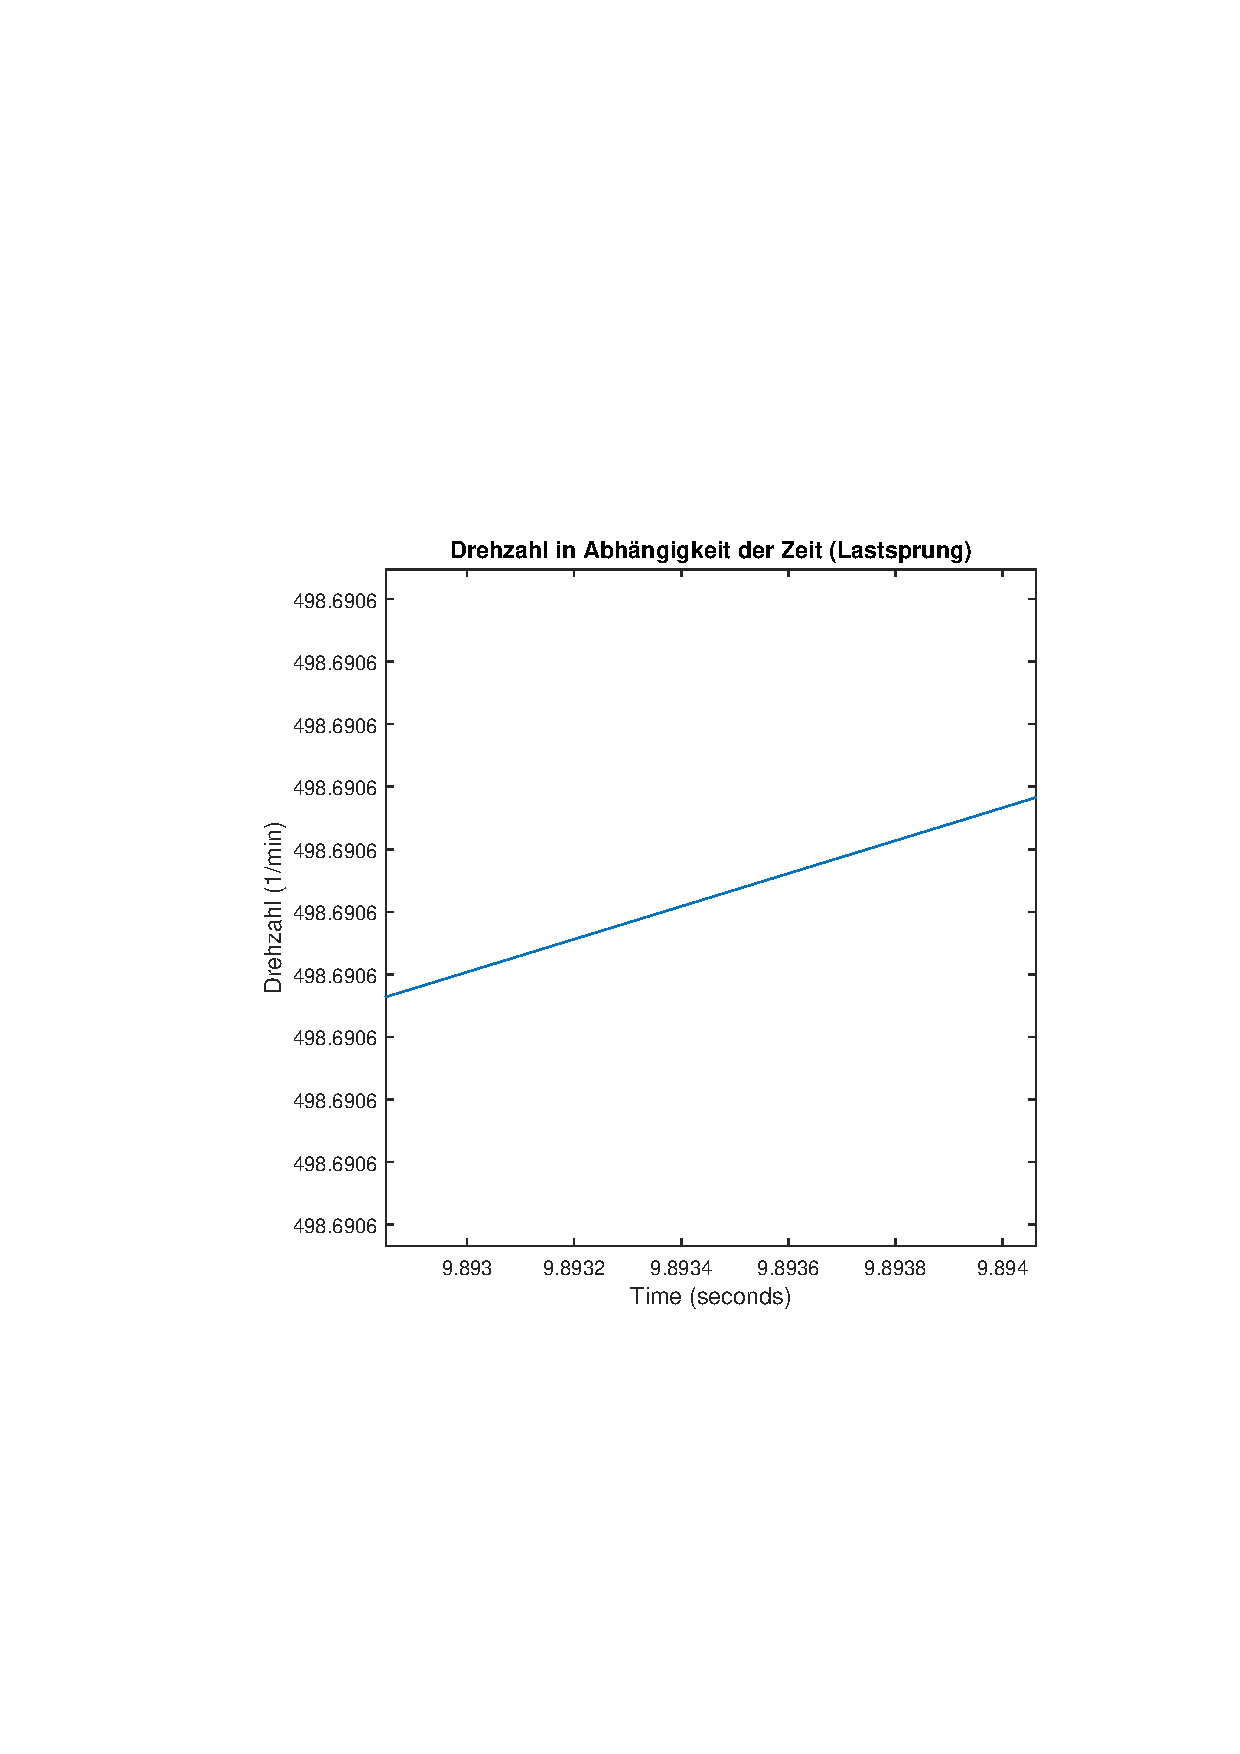
\includegraphics[width=\textwidth]{erg/drehzahl-lastsprung-2.pdf}
\end{minipage}

\section{Simulationsergebnisse am starren Netz}\label{sec:sim-starr-netz}


\section{Aussichten für die Implementierung der Vektorregelung}\label{sec:aussichten-foc}





%%% Local Variables: 
%%% mode: latex
%%% TeX-master: "main"
%%% TeX-open-quote: "\\enquote{"
%%% TeX-close-quote: "}"
%%% LaTeX-csquotes-open-quote: "\\enquote{"
%%% LaTeX-csquotes-close-quote: "}"
%%% End: 
